\documentclass[english,usenames,dvipsnames]{beamer}
\usetheme{default}
\usepackage[utf8]{inputenc}
\usepackage{caption}
\usepackage{appendixnumberbeamer}
\usepackage{babel}
\usepackage{amsmath}
\usepackage{geometry}
\usepackage{bbm}
\usepackage{amsthm}
\usepackage{verbatim}
\definecolor{myred1}{RGB}{255,50,0}
\definecolor{myblue1}{RGB}{0,100,255}
\definecolor{mygreen1}{RGB}{34,139,35}


\title{A Model of Productivity Growth through Creative Destruction by Employee Spinout: Updates}
\author{Nicolas Fernandez-Arias}
\date[May 1, 2018]{May 1, 2018}

\begin{document}
	  
\frame{\titlepage}

\begin{comment}
\begin{frame}{Introduction}
\label{Introduction}
\begin{itemize}
	\item A \textbf{spinout} of a firm is a competing firm founded by a previous employee of the original firm
	\begin{itemize}
		\item E.g. Fairchild semiconductor spinouts form basis of SV \hyperlink{fairchild_spinouts}{\beamerbutton{detail}}
		\item NOT a \emph{spinoff}, which refers to a subsidiary of a company which is broken off from the balance sheet
	\end{itemize}
	\item \textbf{This presentation}: Discuss a candidate model of long-run productivity growth which brings to the fore \textbf{creative destruction by employee spinouts.}
	\begin{itemize}
		\item Adapt the Grossman-Helpman 1991 quality ladders framework to endogenize mass of potential entrants
	\end{itemize}
\end{itemize}
\end{frame}

\begin{frame}{Empirical motivation}
\label{Motivation1}
\begin{itemize}
	\item Technological innovation is major source of long-run growth in labor productivity
	\item Entry contributes substantially to tech innovation, e.g.:
	\begin{itemize}
	\item Empirical decomposition: net job creation higher for young firms
	\item Productivity growth due to entry: over 10-year horizon, 25\% of labor productivity growth accounted by entry in manufacturing (Baily-Bartelsman-Haltiwanger 1996)
	\item Decomposition based on model-based extrapolation from patent citation counts: ~25\% of aggregate productivity growth due to entrants (Akcigit \& Kerr 2017)
	\end{itemize}
	\item Employee spinouts comprise an important, influential subset of entrants
	\begin{itemize}
		\item e.g. Fairchild semiconductor spawned Silicon Valley; earlier, Detroit automakers
		\item In Brazil, employee spinouts account for between 15-30\% of entrants; substantially larger, grow faster, fail less frequently (Muendler et al. 2012)
	\end{itemize}
\end{itemize}
\end{frame}

%%%%%%%%%%%%%%%%%%%%%%%%%%%%%%%%
% Adapt this slide %%%%
%%%%%%%%%%%%%%%%%%%%%%%%%%%%%%%%%
\begin{frame}{Theory: big picture}
\label{theory_big_picture}
\begin{itemize}
	\item Schumpeter 1942, Arrow 1962, etc.: if knowledge is only partially excludable, it will be underproduced in equilibrium because no private benefit to agent incurring costs of production
	\item Intellectual property laws (e.g. patents, copyright, etc.) render knowledge excludable
	\item Patent literature: optimal level of excludability? Dynamic efficiency vs. static monopoly distortion tradeoff (Nordhaus 1967, etc.)
	\item Employee learning and creative destruction by spinout formation implies similar tradeoff
\end{itemize}
\end{frame}


%%%%%%%%%%%%%%%%%%%%%%%%%%%%%%%%%%%%%%%%%%%%%%%
% Add some more citations here if have time %%%%%
%%%%%%%%%%%%%%%%%%%%%%%%%%%%%%%%%%%%%%%%%%%%%
\begin{frame}{Theoretical motivation}
\begin{itemize}
	\item Models of endogenous technological innovation and productivity growth assume knowledge immediately spills over to potential competing entrants
	\begin{itemize}
		\item Grossman \& Helpman 1991 
		\item Akcigit \& Kerr 2017
		\item Acemoglu \& Cao 2015
	\end{itemize}
	\item Models of spinouts are typicaly partial equilibrium and not focused on long-run growth or creative destruction
	\begin{itemize}
		\item Klepper \& Sleeper 2005 - very partial equilibrium 
		\item Franco \& Filson 2006 - no creative destruction  (Pareto efficient)
		\item Franco \& Mitchell 2008 - 
		\item Rauch 2015 - partial equilibrium, no growth or innovation	\item Rossi-Hansberg \& Chatterjee 2012 - no creative destruction
	\end{itemize}
\end{itemize}
\end{frame}

%% NEED TO MAKE SURE THIS IS NESTED IN TRADEOFF SLIDE!%%%%
%%%%%%%%%%%%%%%%%%%%%%%%%%%%%%%%%%%%%%%%%%%%%%%%%%%%%%

\section{Data}
\begin{frame}{Data}
\label{Data}
\begin{itemize}
	\item Have:
	\begin{itemize}
		\item Crunchbase full dataset: free dataset, 100,000+ startups (mostly founded in the last 20 years \hyperlink{crunchbase_founding_dates_coverage}{\beamerbutton{chart}}), information on founders and funding rounds. Some missing data, but more coverage of early stage startups than competing (expensive) datasets
		\item Moments from empirical work: e.g. brain drain in Marx 2015
		\item Survey data from Starr 2017 on prevalence of non-competes
		\item Data on strength of non-compete enforcement from Bishara 2011
	\end{itemize}
	\item Need / want: 
	\begin{itemize}
		\item Previous employment / occupation of founders in Crunchbase dataset. VentureOne has this, but it is not free.
		\item Better industry / product information classification -- need to merge with Crunchbase by firm name
		\item LEHD data would be great for comparing outcomes across different enforcement regions...but hard to come by. 
	\end{itemize}
\end{itemize}
\end{frame}
\end{comment}

%%%%%%%%%%%%%%%%%%%%%%%%%%%%%%%%%%%%%%%%%%
%%% GOING TO NEED TO FIX ALL OF THIS SHIT TOMORROW MORNING!!!%%% 
%%%% BUT I THINK YOU WILL GET SOME USEFUL FEEDBACK! THIS HOPEFULLY WILL NOT BE A DISASTER!!!%%%%

\begin{frame}{Updates - Overview}
	\begin{itemize}
		\item Preliminary proposal for nesting model in general model 
		\begin{itemize}
			\item For now: exogenous shock that makes knowledge public
			\item Potential improvement: immediately allow free entry into R\&D race, but endow spinouts with some extra productivity relative to these entrants. Over time, spinouts drive entrants out of the market.
			\item Very different implications, but hard to observe
		\end{itemize}
		\item Ideas for calibration / identification of parameters
	\end{itemize}
\end{frame}

\begin{frame}{Model overview}
\begin{itemize}
	\item Time $t$ is continuous 
	\item Agents:
	\begin{itemize}
		\item Households 
		\item Intermediate goods firms
		\item Final goods firm 
	\end{itemize}
\end{itemize}
\end{frame}


\section{Model}
\subsection{Overview}
\begin{comment}
\begin{frame}{Model overview}
\begin{itemize}	
	\item Builds on (nests) standard quality ladders model of endogenous growth (Grossman \& Helpman 1991)
	\item Endogenous productivity growth through improved quality of intermediate goods 
	\item Quality improvements result from labor allocated to R\&D
	\item Innovation by creative destruction
	\item \textbf{New ingredient:} R\&D workers learn on the job how to form spinouts which compete in R\&D race with incumbents
\end{itemize}
\end{frame}
\end{comment}

\begin{frame}{Model: Intermediate goods production}
\begin{itemize}
	\item Standard quality ladders model, step size $\lambda > 1$
	\item Continuum of intermediate goods, indexed by $j\in J = [0,1]$
	\item Frontier quality of good $j$ by $q_j$
	\item $x_j$ is amount produced 
	\item Each good produced with technology
	\begin{align*}
	x_j = \bar{q} l_j
	\end{align*}
	where $\bar{q} = \int_0^1 q_j dj$ is the average quality level of the economy
	\item Each good $j$ has monopolist, standard assumptions to guarantee no limit pricing 
	\item Demand (final goods production) CES across goods $j$ implies constant markup
\end{itemize}
\end{frame}

\begin{frame}{Model: R\&D race}
\begin{table}
	\small
	\begin{tabular}{p{0.8\textwidth}}
		\centering
		At time $t$ with average quality $\bar{q}_t$, incumbent in the R\&D race for good $j$ of quality $q_j$ begins with monopoly on good $j$ R\&D \\
		$\downarrow$\\
		\begin{itemize}
			\item 	Hires R\&D labor; at rate $\nu (q_j/\bar{q}_t)^{-1}$ per unit of R\&D labor hired, employees learn, adding to mass of potential entrants (\textbf{scaling factor $(q_j/\bar{q}_t)^{-1}$ for BGP})) \\
			\textcolor{mygreen1}{\item Simultaneously, with arrival rate $\theta$, ``knowledge spillover" shock hits $\rightarrow$ \textbf{free entry} into R\&D race}
		\end{itemize}
	
		$\downarrow$\\
		At some point, either an incumbent or an entrant firm wins the race, and obtains a monopoly on production and R\&D on good $j$ of quality $\lambda q_j$
	\end{tabular}
\end{table}
\end{frame}

\begin{frame}{Model: R\&D technology}
\begin{itemize}
	\small
	\item Consider an intermediate $j$ with relative quality $\tilde{q} = q / \bar{q}$
	\item \textbf{Scaling assumption for BGP:} flow cost of $\tilde{q}z$ units of labor yields $z$ units of effective labor 
	\item $z$,$\hat{z}$ units of R\&D effort by incumbent and entrant respectively yields victory in the R\&D race at Poisson rate
	\begin{align*}
	R(z) &= \chi z \phi(z) \\
	\hat{R}(\hat{z};\bar{z}) &= \hat{\chi} \hat{z} \eta(\bar{z}) 
	\end{align*}
	where $\bar{z} = \int_0^{m} \hat{z}(m')dm'$ is total good-$j$ R\&D effort by entrants.
	\item Entrant $m'$ can perform $\hat{z}\le\xi$ units of R\&D effort (equilibrium does not pin down; look for equilibria where $\hat{z}(m') \in \{0,\xi \}$)
	\item Aggregate rate of innovations:
	\begin{align*}
	\tau = \chi z \phi(z) + \hat{\chi} \bar{z} \eta(\bar{z})
	\end{align*}
\end{itemize}
\end{frame}

\begin{frame}{Model: R\&D technology - congestion}
\begin{itemize}
	\item The reduced-form functions $\phi(z),\eta(z)$ capture diminishing returns and congestion in the R\&D race, repsectively
	\item As such, assume $\phi(z),\eta(z)$ decreasing, $z\phi(z),z\eta(z)$ increasing
	\item For the incumbent, $\phi(z)$ captures \textit{individual} decreasing returns in the R\&D technology
	\item For the entrants, $\eta(z)$ captures \textit{aggregate} decreasing returns due to the possibility that different entrants use the same approach 
	\item Cross-congestion:
	\begin{itemize}
		\item Incumbent and entrants do not congest each other (as in other models of innovation by entrants and incumbents, c.f. Acemoglu \& Cao 2015, Akcigit \& Kerr 2017)
		\item Adds tractability and reflects empirical fact that spinouts often attempt different approaches
		\item Can be relaxed
	\end{itemize}
\end{itemize}
\end{frame}

\begin{frame}{Intermediate goods firms optimization: incumbent static optimization}
\begin{itemize}
	\footnotesize
	\item Static optimization in product market: CES final goods production implies constant markup
	\item Regardless of the aggregate supply of labor, have
	\begin{align*}
		\bar{w} &= \tilde{\beta} \bar{q}  \\
		\tilde{\beta} &= \beta^{\beta} (1-\beta)^{2-2\beta} 
	\end{align*}
	where $L^F$ is labor allocated to final goods production. 
	\item Taking as given research labor allocation $L^{RD}$, have closed forms for $L^F,L^I$ and static profits $\pi(q)$ for an incumbent with technology $q$,
	\begin{align*}
	L^F &= \frac{\beta(1-L^{RD})}{\beta + (1-\beta)^2} \\
	L^I &= 1 - L^{RD} - L^F \\
	\pi &= \beta(1-\beta)^{\frac{2-\beta}{\beta}} \tilde{\beta}^{-1} L^F q
	\end{align*}
\end{itemize}
\end{frame}

\begin{frame}{Intermediate goods firms optimization: incumbent R\&D decision}
\begin{itemize}
	\item HJB equation for incumbent:
	\footnotesize
	\begin{align*}
	(\rho + \overbrace{\hat{\chi} \bar{z}(q,m,t)\eta(\bar{z}(q,m,t))}^{\text{Entrant innovation rate}}) V(q,m,t) &= \overbrace{\pi q}^{\text{Flow profits}} + \overbrace{V_t(q,m,t)}^{\text{Changing aggregate state}} \\ 
	 +  \overbrace{\nu \bar{z}(q,m,t) V_m(q,m,t)}^{\text{Knowledge spillovers from entrant R\&D}} & + \textcolor{mygreen1}{\overbrace{\theta \Big(V(q,M,t) - V(q,m,t)\Big)}^{\text{Knowledge becomes public}}}\\
	 + \max_{\textcolor{myred1}{z}} \Big\{\underbrace{\chi \textcolor{myred1}{z}\phi(\textcolor{myred1}{z})}_{\text{Arrival rate of R\&D victory}} &\textcolor{myblue1}{\overbrace{\Big(V(\lambda q,0,t)-V(q,m,t)\Big)}^{\text{NPV of successful innovation}}} \\
	 -\underbrace{\textcolor{myred1}{z}(q/\bar{q}_t)}_{\text{R\&D labor}} \big(\underbrace{w(q,m,t)}_{\text{R\&D wage}} - & \overbrace{\nu (q/\bar{q}_t)^{-1} V_m(q,m,t)}^{\text{Knowledge spillovers from own R\&D}}\big)\Big \}
	\end{align*}
\end{itemize}
\end{frame}

\begin{frame}{Intermediate goods firms optimization: entrant R\&D decision}
\begin{itemize}
	\item HJB equation for entrant: 
	\footnotesize
	\begin{align*}
	(\rho +  \overbrace{\hat{\chi} \bar{z}(q,m,t)\eta(\bar{z}(q,m,t)+ )}^{\text{Entrant innovation rate}}) & W(q,m,t) = \overbrace{W_t(q,m,t)}^{\text{Changing aggregate state}} \\
	 + \overbrace{\nu \bar{z}(q,m,t) W_m(q,m,t)}^{\text{Knowledge spillovers from entrant R\&D}} &+ \textcolor{mygreen1}{\overbrace{\theta \Big(W(q,M,t) - W(q,m,t)\Big)}^{\text{Knowledge becomes public}}} \\
	 + \max_{\textcolor{myred1}{z}} \Big \{ \overbrace{\hat{\chi} {\textcolor{myred1}{z}} \eta(\bar{z}(q,m,t))}^{\text{Arrival rate of R\&D victory}} & \textcolor{myblue1}{\overbrace{\Big( V(\lambda q,0,t) - W(q,m,t) \Big)}^{\text{NPV of successful innovation}}} \\
	& - \underbrace{\textcolor{myred1}{z}(q/\bar{q}_t)}_{\text{R\&D labor}} \underbrace{w(q,m,t)}_{\text{R\&D wage}}  \Big\}
	\end{align*}
\end{itemize}
\end{frame}

\begin{frame}{Model: Households}
\begin{itemize}
	\item Unit mass continuum of risk-neutral households indexed by $i\in I =[0,1]$, each with objective
	\begin{align*}
	U = \int_0^{\infty}\exp(-\rho t)c(t)dt
	\end{align*}
	where $c(t)$ is final goods consumption at $t$.
	\item Instantaneous borrowing and lending at interest rate $r$; $r = \rho$ in equilibrium
	\item Individual $i$ supplies labor to final goods production $\ell^F_i (t)$, intermediate good production $\ell^I_i (t)$ and R\&D $\ell_i^{RD} (t)$ such that 
	\begin{align*}
	\ell_i^F(t)+ \ell_i^I(t) + \ell_i^{RD}(t) = 1
	\end{align*}
	\item Aggregate labor market satisfies (where $L^k(t) = \int_I \ell_i^k(t) idi$ for $k\in\{F,I,RD\}$)
	\begin{align*}
	L^F(t) + L^I(t) + L^{RD}(t) = 1
	\end{align*}
\end{itemize}
\end{frame}

\begin{frame}{Household optimization timeline}
\begin{table}
\begin{tabular}{p{0.8\textwidth}}
	\centering
	Worker $i$ allocates labor to R\&D, intermediate and final goods production \\
	$\downarrow$\\
	While performing R\&D for some good $j$ of relative quality $\tilde{q}_j$, receives learning shock with Poisson intensity $\nu \tilde{q}_j^{-1}$ per flow unit of R\&D labor supplied to $j$
	$\downarrow$\\
	Provided it is still profitable, he opens entrant R\&D lab performing R\&D effort $\xi$ and competing in developing the next step of good $j$
\end{tabular}
\end{table}
\end{frame}

\begin{frame}{Household optimization}
\small
\begin{itemize}
\item Workers indifferent between occupations (Final goods production, intermediate goods production, R\&D). 
\item \textbf{For production:} Indifference requires requires same wage in final goods and intermediate goods production: $w_t^I = w_t^F = \bar{w}$.
\item \textbf{For R\&D:} Indifference now requires \textbf{total compensation} from R\&D -- including \textbf{expected value of knowledge earned} -- to be equal to $\bar{w}$, i.e.
\begin{align*}
w(m,t) + \nu W(m,t) &= \bar{w}_t
\end{align*}
where $W(m,t)$ is the value at time $t$ of the knowledge to open an entrant in a good which is currently in state $m$
\end{itemize}
\end{frame}

\begin{frame}{Model: Final good production}
\begin{itemize}
	\item Final good is produced using labor and a continuum of intermediate goods $j\in[0,1]$ with production technology
	\begin{align*}
	X(t) &= L(t)^{\beta}\Bigg(\Big(\int_0^1 q_j(t)^\beta 
	x_j(t)^{1-\beta}dj \Big)^{1/(1-\beta)}\Bigg)^{1-\beta} \\
	&=  L(t)^{\beta}\int_0^1 q_j(t)^\beta x_j(t)^{1-\beta}dj
	\end{align*}
	where $q_j$ is quality, $x_j$ is quantity
	\item Restricts labor share to be related to markup $\mu = 1/(1-\beta)$
	\item Can relax this using Grossman et. al 2016
	\item CRS implies zero profits so no need to consider ownership
\end{itemize}
\end{frame}


\begin{frame}{Aggregation: Kolmogorov Forward Equation}
\begin{itemize}
	\small
	\item Define $d\mu(q,m,t)$ as the distribution of intermediate goods $j$ across states $(q,m)$ at time $t$
	\item Kolmogorov Forward Equation (somewhat heuristic) 
	\begin{align*}
	\mu_t(q,m,t) &= \overbrace{-\frac{d}{dq} (a^q(q,m,t) \mu(q,m,t))}^{\text{Drift in $q$}} - \overbrace{\frac{d}{dm} (a^m(q,m,t) \mu(q,m,t))}^{\text{Drift in $m$}} \\ 
				 & - \underbrace{\tau(q,m,t)\mu(q,m,t)}_{\text{Innovation arrival: jump } (q,m) \to (\lambda q,0)} \\
				 & + \underbrace{\mathbbm{1}_{\{m = 0 \}}\lambda^{-1} \int \tau(\lambda^{-1}q,m',t) d\mu(\lambda^{-1}q,m',t)}_{\text{Innovation arrival: jump } (\lambda^{-1}q,m') \to (q,0)}
	\end{align*}
	\item $a^q(q,m,t),a^m(q,m,t)$ are drift in $q,m$ direction, respectively, computed from $z(q,m,t)$ and $\bar{z}(q,m,t)$
	\item Last term for $m = 0$ arises because receiving inflows from $(\lambda^{-1}q,m')$ for all $m'$ 
	\item Factor $\lambda^{-1}$ due to $d(\lambda q) = \lambda dq$
\end{itemize}
\end{frame}

\subsection{Equilibrium}
\begin{frame}{Recursive BGP Equilibrium}
\begin{itemize}
	\footnotesize
	\item For notation, below I sometimes omit dependence of functions on $(q,m,t)$
	\item Growth rate $g$ of average quality $\bar{q}_t$, value functions $V,W$, individual R\&D policies $z$ and $\hat{z}$, aggregate R\&D intensity $\tau$, entrant R\&D intensity $\bar{z}$, prices of intermediate goods, final and intermediate goods wage $\bar{w}$, and a distribution $d\mu$ such that: 
	\begin{itemize}
		\footnotesize
		\item Intermediate goods firms and final goods firms statically optimize production decisions
		\item Value functions $V,W$ solve HJB eqs, individual policy functions optimal given value functions
		\item Distribution $\mu(q,m,t)$ satisfies KF equation (time dependent, haven't shown)
		\item Final and intermediate goods wage satisfy $\bar{w} = \Gamma(\beta)$
		\item R\&D wages satisfy indifference condition $w(q,m,t) + \nu (q/\bar{q}_t)^{-1} W(q,m,t) = \bar{w}$
		\item Labor resource constraint: $L^F + L^I + L^{RD} = 1$
		\item Growth is constant at $g$, and consistent with R\&D policy functions and distribution $\mu(q,m,t)$: $g = (\lambda -1) \int \tau(q,m,t) (q/\bar{q}_t) d\mu(q,m,t)$
	\end{itemize} 
\end{itemize}
\end{frame}

\begin{frame}{Finding a BGP}
\begin{itemize}
	\item Recall that in equilibrium, $w(q,m,t) = \tilde{\beta}\cdot\bar{q}_t - \nu W(q,m,t)$
	\item Taking this into account, in equilibrium the following holds: 
	\footnotesize
	\begin{align*}
	(\rho + \overbrace{\hat{\chi} \bar{z}(q,m,t)\eta(\bar{z}(q,m,t))}^{\text{Entrant innovation rate}}) V(q,m,t) = \overbrace{\pi q}^{\text{Flow profits}} &+ \overbrace{V_t(q,m,t)}^{\text{Changing aggregate state}} \\ 
	+  \overbrace{\nu \bar{z}(q,m,t) V_m(q,m,t)}^{\text{Knowledge spillovers from entrant R\&D}}  &\\
	+ \max_{\textcolor{myred1}{z}} \Big\{\underbrace{\chi \textcolor{myred1}{z}\phi(\textcolor{myred1}{z})}_{\text{Arrival rate of R\&D victory}} &\overbrace{\textcolor{myblue1}{\Big(V(\lambda q,0,t)-V(q,m,t)\Big)}}^{\text{NPV of successful innovation}} \\
	-\underbrace{\textcolor{myred1}{z}(q/\bar{q}_t)}_{\text{R\&D labor}} \underbrace{\big(\tilde{\beta}\cdot\bar{q}_t - \nu (q/\bar{q}_t)^{-1}W(q,m,t)}_{\text{Equilibrium R\&D wage}} - & \overbrace{\nu (q/\bar{q}_t)^{-1} V_m(q,m,t)}^{\text{Knowledge spillovers from own R\&D}}\big)\Big \} 
	\end{align*}
\end{itemize}
\end{frame}

\begin{frame}{Finding a BGP: Guess and verify}
\begin{itemize}
	\item Guess and verify: abusing notation, value of \textbf{incumbent} is $V(q,m,t) = qV(m)$, value of \textbf{entrant} is $W(q,m,t) = qW(m)$
	\item Given these guesses, makes sense to guess $\bar{z}(m,q,t) = \bar{z}(m) = \xi \min(m,M)$ for some $M > 0$
	\item Plugging guess into incumbent HJB yields: for $m < M$,
	\begin{align*}
	(\rho +  \hat{\chi}\xi m \eta(\xi m) ) V(m) &= \pi + \textcolor{mygreen1}{\overbrace{\theta \Big(V(M) - V(m) \Big)}^{\text{Knowledge becomes public}}} + \nu \xi m V'(m) \\
	&+ \max_{z} \Big\{ \chi z \phi(z) (\lambda V(0) - V(m))   \\
	&- z (\bar{w} - \nu (W(m) + V'(m)) \Big\}
	\end{align*}
	where $\bar{w} = \tilde{\beta}$. 
	\item Boundary condition: $V'(m) = 0$ for $m \ge M$
\end{itemize}
\end{frame}

\begin{frame}{Finding a BGP: Guess and verify (cont.)}
\begin{itemize}
	\small
	\item Similarly, HJB equation for entrant becomes: for $m < M$, 
	\small
	\begin{align*}
	(\rho + \hat{\chi}\xi m \eta(\xi m) ) W(m) &= \textcolor{mygreen1}{\overbrace{\theta \Big(W(M) - W(m)\Big)}^{\text{Knowledge becomes public}}} + \nu \xi m W'(m) \\
	&+ \max_{z} \Big\{ \chi z \eta(\xi m) (\lambda V(0) - W(m))   \\
	&- z (\bar{w} - \nu W(m) \Big\}
	\end{align*}
	\item Boundary condition: $W(M) = 0$ 
	\item Equilibrium $M$ pinned down by free-entry condition
	\begin{align*}
	\eta(M) \lambda V(0) = \bar{w}
	\end{align*}
\end{itemize}
\end{frame}

\begin{comment}

\begin{frame}{Finding BGP: Solving HJBs numerically (I)}
\begin{enumerate}
	\item NEED TO FIX - still working on this
	\item Guess R\&D wage $w(\cdot)$
	\item Solve for $V(\cdot),M$ given $W(\cdot)$: 
	\begin{enumerate}
		\item Guess $V(0)$
		\item Free entry condition and $V(0)$ determine $M$
		\item $M$ determines entrant strategy: $z^E(m) = \xi \min(m,M)$
		\item Integrate backward HJB and boundary condition $V'(M) = 0$ 
		\item Check that $V(0)$ in solution is the same as guess; if not, update and return to 2.1
		\item Convergence guaranteed if mapping from $V(0)$ guess to $V(0)$ output is continuous and monotonic, both of which seem correct (but I haven't checked yet, working on code).
	\end{enumerate}
	\item Using $M$ computed from the previous step, solve for implied $W(\cdot)$
	\begin{enumerate}
		\item Integrate entrant HJB backward starting from boundary condition $W(M) = 0$
		\item Denote resulting function by $\hat{W}(m)$ 
		\item Check $d(W,\hat{W})$ using some metric; if not converged, update guess and return to Step 1. 
	\end{enumerate}
\end{enumerate}
\end{frame}

\begin{frame}{Finding a BGP: Stationary distribution $\mu(m)$}
\begin{itemize}
	\small
	\item No need to keep track of aggregate distribution across $q$
	\item Conjecture that a BGP exhibits a stationary distribution $d\mu(m,t) = d\mu(m)$
	\item For $m > 0$, the distribution $d\mu(m)$ will have no mass points, therefore its density $\mu(m)$ is well defined and satisfies the Kolmogorov Forward Equation: 
	\begin{align*}
		0 = -\frac{d}{dm} (a(m) \mu(m)) - \tau(m)\mu(m)  
	\end{align*}
	\item For $m > M$, have $a(m)$ and $\tau(m)$ constant, so the above becomes 
	\begin{align*}
		\mu'(m) = -\frac{\tau(M)}{a(M)} \mu(m)
	\end{align*}
	\item Solution given by $\mu(m) = \mu(M)e^{-(\tau(M) / a(M))(m-M)}$ for $m \ge M$
	\item Probably solve the rest numerically
\end{itemize}
\end{frame}

\begin{comment}
\begin{frame}{Finding a BGP: Stationary distribution $\mu(m)$ (cont.)}
\begin{itemize}
	\item Setting $m=M$ yields $\mu(M) = K$
	\item Integrate numerically to compute $\mu(m)$ for $m < M$
	\item Compute total mass of $m > 0$ by integrating numerically
	\begin{align*}
		M_+ = \int_0^{\infty} \mu(m) dm
	\end{align*}
	\item Finally, compute total rate at which mass 
\end{itemize}
\end{frame}

\begin{frame}{Finding a BGP: Algorithm}
\begin{itemize}
	\item The numerical algorithm I propose for computing a BGP is as follows:
	\begin{enumerate}
		\item Guess $L^F$, the labor supply to final goods production
		\item This guess pins down equilibrium profit flow $\pi$ and final goods / intermediate goods wage $\bar{w}$
		\item Given these, solve HJBs numerically using iterative procedure described above
		\item Next, solve KF equation to compute stationary distribution $\mu(m)$
		\item Using $\mu(m)$ and policy functions from previous step, integrate to compute aggregate labor demand 
		\item Check that aggregate labor demand is equal to the unit labor supply. If not, adjust guess for $L^F$ and return to Step 1.
		\item Finally, integrate innovation arrival rates to compute $g = (\lambda-1)\int \tau(m) d\mu(m)$
	\end{enumerate}
\end{itemize}
\end{frame}


\begin{comment}

\begin{frame}{Challenges: obtaining BGP}
\begin{itemize}
	\item In usual Neo-Schumpeterian growth models, technology scaling assumptions guarantee that arrival rate of innovations is independent of $q$
	\item Aggregate growth rate can be computed without reference to distribution of goods across different quality levels
	\item My model does not have this property, stemming from the worker indifference condition $w(q,m) = \bar{w} - \nu W(q,m)$
	\item Other models of spinouts generally have this property as well
\end{itemize}
\end{frame}



\begin{frame}{BGP with $\hat{\chi} = 0$}
\begin{itemize}
	\small
	\item To see a case with a BGP, consider the case where $\hat{\chi} = 0$ (could also consider case of free entry)
	\item This implies $m=0$, so $m$ no longer a state variable
	\item Wage satisfies $w(q) = \bar{w}$ since workers do not learn on the job
	\item Model becomes a standard quality ladders endogenous growth model with no entry 
	\begin{align*}
	(\rho - g)V(\tilde{q}) &= \pi \tilde{q} - g\tilde{q}V'(\tilde{q}) \\
	& + \max_{z} \Big z\chi\phi(z) {\Big(V(\lambda\tilde{q})-V(\tilde{q})\Big)} - \tilde{q} z \bar{w}\} 
	\end{align*}
\end{itemize}
\end{frame}

\begin{frame}{BGP with $\hat{\chi} = 0$}
\begin{itemize}
	\item Guess and verify $V(\tilde{q}) = V_0 \tilde{q}$: 
	\begin{align*}
	(\rho - g) V_0 \textcolor{myred1}{\tilde{q}} = \tilde{\pi}\textcolor{myred1}{\tilde{q}} - g\textcolor{myred1}{\tilde{q}}V_0 + \max_z \Big\{ z\chi \phi(z) \Big(\lambda \textcolor{myred1}{\tilde{q}}V_0 - \textcolor{myred1}{\tilde{q}} V_0 \Big)- \textcolor{myred1}{\tilde{q}} z \bar{w}  \Big\}
	\end{align*}
	\item FOC for $z$
	\begin{align*}
	\chi((\phi(z) + z\phi ' (z) (\lambda -1)V_0 = \bar{w}
	\end{align*} 
	\item Does not involve $q$ so gives $z^*(q) = z^*$:
	\begin{align*}
	z^* = \Big( \frac{\chi(\lambda-1)V_0}{\bar{w}} \Big)^{\frac{1}{p}}
	\end{align*}
\end{itemize}
\end{frame}

\begin{frame}{BGP with $\hat{\chi} = 0$}
\begin{itemize}
	\item Cancelling $\tilde{q}$ terms confirms guess, get expression for $V_0$ given by
	\begin{align*}
	(\rho + \chi z^* \phi(z^*)(1-\lambda))  V_0 = \tilde{\pi} - z^* \bar{w}
	\end{align*}
	\item Plugging in expression for $z^*$ yields 
	\begin{align*}
	V_0 = \frac{\tilde{\pi} - \Big( \frac{\chi(\lambda-1)V_0}{\bar{w}} \Big)^{\frac{1}{p}} \bar{w}}{\rho + \Big( \frac{\chi(\lambda-1)V_0}{\bar{w}} \Big)^{\frac{1}{p} - 1}}
	\end{align*}
	\item RHS is continuous and, for $p \in (0,1)$, strictly decreasing in $V_0$
	\item Intermediate value theorem implies existence and uniqueness of solution $V_0$, confirming guess 
\end{itemize}
\end{frame}

\begin{frame}{Efficiency}
\begin{itemize}
	\small
	\item Worker indifference condition implies firm compensated (in expectation) for profits of future spinouts
	\item Franco-Filson 2006 logic suggests this may imply Pareto efficiency
	\item However, this ignores creative destruction
	\item Spinouts may reduce value of incumbent-worker pair by destroying monopoly power
	\item Equilibrium wage discount does not fully compensate R\&D firm for knowledge produced
	\item So model exhibits standard Schumpeterian inefficiency from R\&D firms not fully appropriating the returns to their investments
	\item Also standard: potential for inefficiently high creative destruction due to entrants not internalizing their ``business stealing" effect
\end{itemize}
\end{frame}

\section{Extensions}
\begin{frame}{Next steps}
\begin{itemize}
	\item Existence and uniqueness of BGP; maybe closed forms for certain functional forms? 
	\item Implement proposed algorithm for solving model numerically
	\item Calibrate, test the model
	\begin{itemize}
		\item Microeconometric facts about employee spinouts from e.g., Starr et. al "Screening spinouts"
		\item Klepper-Sleeper 2005
	\end{itemize}
	\item Potential extensions
	\begin{itemize}
		\item Learning and entrepreneurship decisions 
		\item Different step sizes for incumbents and entrants 
		\item Cross-congestion
		\item Labor contracts: non-competes
	\end{itemize}
\end{itemize}
\end{frame}



\begin{frame}{Identification}
	\item What fraction of entrants are spinouts?
	\begin{itemize}
		\item Employer-employee matched data (LEHD, Brazilian data, German data): identify spinouts as in Muendler et al. 2012
		\item Establishment level data (same datasets): identify entrant firms, rate of entry, etc.
		\item \textbf{Problem:} entrants in data are not just creative destruction. Will overestimate number of entrants, hence overestimate role of within-industry spinouts in entry. 
		\item \textbf{Problem:} firms have more than one product. \textbf{Solution:} 
	\end{itemize}
	\item What fraction of winners of R\&D race are spinouts?
	\begin{itemize}
		\item How to identify winners of R\&D race in the data? (1) entrants that are still around after $n$ years, for some $n$; (2) entrants that grow to a certain percentile in the firm-size distribution  
	\end{itemize}
	\item Average R\&D expenditure given the state $m$ of an industry?
\end{frame}
\end{comment}

\begin{frame}{Alternative nesting of model}
\begin{itemize}
	\item The above feels ad-hoc. I am arbitrarily restricting entrants until a reduced form shock occurs.
	\item Another possibility: endow employees who learn on the job with a more efficient R\&D
	\item Specifically, if $\bar{z}$ is total innovation effort by entrants (spinouts or not), the R\&D production functions are (for spinouts, non-spinouts, respectively):
	\begin{align*}
		\hat{R}_S (\hat{z}_S; \bar{z}) &= \hat{\chi}_S \hat{z}_S \eta(\bar{z}) \\ 
		\hat{R}_E (\hat{z}_E; \bar{z}) &= \hat{\chi}_E \hat{z}_E \eta(\bar{z}) 
	\end{align*}
	\item Nests standard model when $\hat{\chi}_E \ge \hat{\chi}_S$
\end{itemize}
\end{frame}

\begin{frame}{Identification}
\begin{itemize}
	\item Specialize $\phi(z) = \eta(z) = z^{-\psi}$
	\item Parameters in baseline model: $\{\beta,\rho,\lambda,\chi,\psi,\nu,\xi,\theta\}$
	\item No closed forms so even when a certain moment ``identifies" a parameter, I will have to do identification with indirect inference. 
	\item General parameters: $\{\rho,\beta\}$
	\item R\&D parameters: $\{\psi,\lambda, \chi\}$
	\item Spinout parameters: $\{ \nu,\xi,\theta \}$
	\begin{itemize}
		\item Empirical component of my paper
		\item Attempt to identify using data on spinouts and creative destruction (details on next slide)
	\end{itemize}
\end{itemize}
\end{frame}

\begin{frame}{Identification: $\rho, \beta$}
\begin{itemize}
	\item Calibrating $\rho$:
	\begin{itemize}
		\item Agents in model are risk-neutral $\Rightarrow$ Interest rate = $\rho$
		\item To get realistic interest rate, have to assume unrealistic discount factor
	\end{itemize}
	\item Calibrating $\beta$:
	\begin{itemize}
		\item In model, $\beta$ determines elasticity of substitution across intermediate goods varieties labor share of final goods firm value-added
		\item In my model, makes more sense to have realistic markups than realistic labor share of final goods production
		\item Idea: follow AK 2017 in identifying based on profit / sales ratio (of, say, incumbent firms)
		\item How to interpret final goods labor in this model if I think of intermediate goods as actually goods? Retail workers? Does this pose a problem given that I have required R\&D workers to be indifferent? 
	\end{itemize}
\end{itemize}
\end{frame}

\begin{frame}{Identification: R\&D parameters $\psi, \lambda, \chi$}
\begin{itemize}
	\item Difficult to disentangle using data generated from a single BGP 
	\item Setting $\psi$:
	\begin{itemize}
		\item Literature has identified using (1) elasticity of R\&D spending to tax changes, (2) elasticity of patents to R\&D spending
		\item Both suggest $\psi \approx 2$
	\end{itemize}
	\item Calibrating $\lambda$:
	\begin{itemize}
		\item Literature has typically tried various values (approx 1.2) and checked robustness
		\item AK 2017: identify based on patent citation distribution
	\end{itemize}
	\item Calibrating $\chi$:
	\begin{itemize}
		\item Given other R\&D parameters, can identify from measures of R\&D intensity  
	\end{itemize}
\end{itemize}
\end{frame}

\begin{frame}{Identification of spinout parameters}
\begin{itemize}
	\item Identifying $\theta$:
	\begin{itemize}
		\item Idea: fraction of existing firms which are spinouts? 
		\item Idea: fraction of startups which are spinouts?
	\end{itemize}
	\item What fraction of winners of R\&D race are spinouts?
	\begin{itemize}
		\item How to identify winners of R\&D race in the data? (1) entrants that are still around after $n$ years, for some $n$; (2) entrants that grow to a certain percentile in the firm-size distribution  
	\end{itemize}

	\item Employer-employee matched data (LEHD, Brazilian data, German data): identify spinouts as in Muendler et al. 2012
	\item Establishment level data (same datasets): identify entrant firms, rate of entry, etc.
	\item \textbf{Problem:} entrants in data are not just creative destruction. Will overestimate number of entrants, hence overestimate role of within-industry spinouts in entry. 
	\item \textbf{Problem:} firms have more than one product.
	\item Average R\&D expenditure given the state $m$ of an industry?

	\item What fraction of winners of R\&D race are spinouts?

	\item Average R\&D expenditure given the state $m$ of an industry? 
\end{itemize}
\end{frame}

\begin{frame}{Identification of Alternative Nesting}
\begin{itemize}
	\small
	\item To the extent that $\hat{\chi}_S > \hat{\chi}_E$, the model has predictions on:
	\begin{enumerate}
		\item The fraction of firms which started out as spinouts vs. ordinary entrants
		\item How the likelihood of successful overtaking by a spinout increases with the time since the last innovation 
		\item Stark model will likely have trouble matching data - eventually, create some attenuation by adding heterogeneity in R\&D productivity of both spinouts and entrants...but I am getting ahead of myself.
	\end{enumerate}
	\item If I can come up with a proxy for $m$ or ``time since last innovation" in the data, I can identify this mechanism.  
	\item Need a proxy for "how many products are currently being developed that compete with this product". 
	\item Idea: Extend Muendler 2012 logic. Entrants that hire many employees of an existing firm are classified as spinouts. But entrants that hire some employees are still more likely to be competing firms than entrants that hire no employees. 
	\item \textbf{I can distinguish much more reliably between these two using VentureSource data. }
	\item Ideas in the literature for identifying these things? 
\end{itemize}
\end{frame}

\begin{frame}{Identification: next steps}
\begin{itemize}
	\item Previous slides were for baseline model which assumed same R\&D technology for incumbents and entrants
	\item May be helpful to allow $\psi,\lambda,\chi$ to differ between incumbents and entrants
	\begin{itemize}
		\item Empirical evidence suggests incumbents focus on incremental innovations while entrants focus on more substantial innovations
		\item Probably reasonable to assume $\psi$ the same for incumbents and entrants, but can do robustness checks.
		\item $\chi,\lambda$ should be allowed to vary: can identify using patent data as in AK 2017. 
	\end{itemize}
\end{itemize}
\end{frame}


% Appendix for figures

\appendix

\captionsetup[figure]{labelformat=empty}

\begin{frame}{Spinouts of Fairchild Semiconductor}
\label{fairchild_spinouts}
\hyperlink{Introduction}{\beamerbutton{back}}
\begin{figure}
	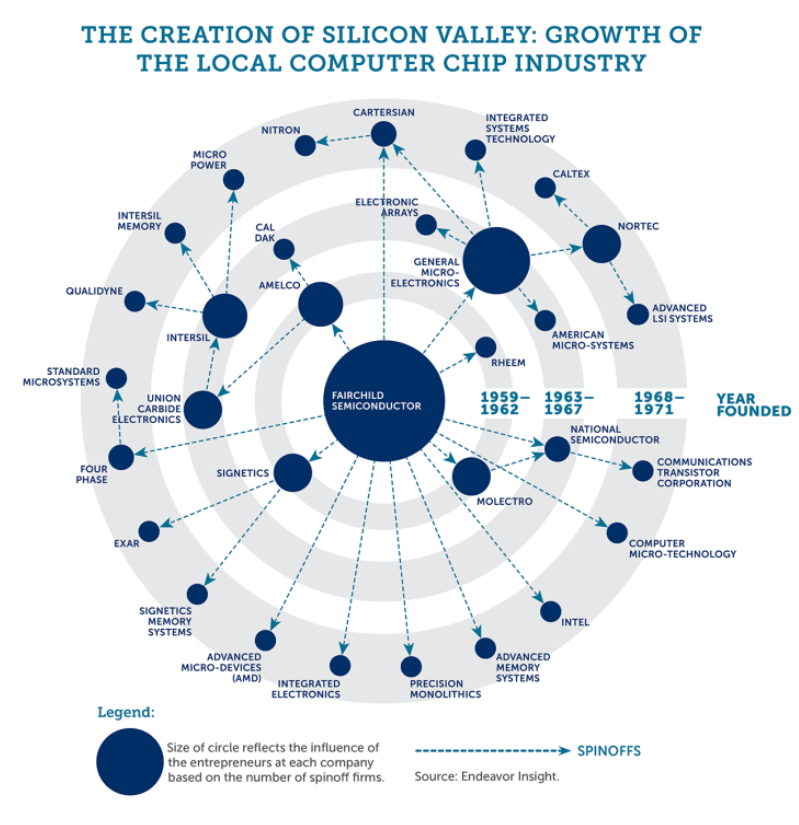
\includegraphics[scale=0.38]{figures/fairchild_spinouts}
	\caption{Source: Endeavor Insights}
\end{figure}
\end{frame}









\end{document}